% Gemini theme
% https://github.com/anishathalye/gemini

\documentclass[final]{beamer}

% ====================
% Packages
% ====================

\usepackage[T1]{fontenc}
\usepackage{lmodern}
\usepackage[size=custom,width=120,height=72,scale=1.0]{beamerposter}
\usetheme{gemini}
\usecolortheme{gemini}
\usepackage{graphicx}
\usepackage{booktabs}
\usepackage{tikz}
\usepackage{pgfplots}
\pgfplotsset{compat=1.14}
\usepackage{anyfontsize}

% ====================
% Lengths
% ====================

% If you have N columns, choose \sepwidth and \colwidth such that
% (N+1)*\sepwidth + N*\colwidth = \paperwidth
\newlength{\sepwidth}
\newlength{\colwidth}
\setlength{\sepwidth}{0.025\paperwidth}
\setlength{\colwidth}{0.3\paperwidth}

\newcommand{\separatorcolumn}{\begin{column}{\sepwidth}\end{column}}

% ====================
% Title
% ====================

\title{Modelling The Rubik's Cube}

\author{Tony X \inst{1} \and Pesara A \inst{1} \and Zeyn J \inst{1}}

%\institute[shortinst]{\inst{1} Some Institute \samelineand \inst{2} Another Institute}
\institute[shortinst]{\inst{1} McMaster University}
% ====================
% Footer (optional)
% ====================

%\footercontent{
%  \href{https://www.example.com}{https://www.example.com} \hfill
%  ABC Conference 2025, New York --- XYZ-1234 \hfill
%  \href{mailto:alyssa.p.hacker@example.com}{alyssa.p.hacker@example.com}}
% (can be left out to remove footer)

% ====================
% Logo (optional)
% ====================

% use this to include logos on the left and/or right side of the header:
% \logoright{\includegraphics[height=7cm]{logo1.pdf}}
% \logoleft{\includegraphics[height=7cm]{logo2.pdf}}

% ====================
% Body
% ====================

\begin{document}

\begin{frame}[t]
\begin{columns}[t]
\separatorcolumn

\begin{column}{\colwidth}

  \begin{block}{Abstract}

   % Some block contents, followed by a diagram, followed by a dummy paragraph.

%%    \begin{figure}
%%      \centering
%%      \begin{tikzpicture}[scale=6]
%%        \draw[step=0.25cm,color=gray] (-1,-1) grid (1,1);
%%        \draw (1,0) -- (0.2,0.2) -- (0,1) -- (-0.2,0.2) -- (-1,0)
%%          -- (-0.2,-0.2) -- (0,-1) -- (0.2,-0.2) -- cycle;
%%      \end{tikzpicture}
%%      \caption{A figure caption.}
  %%  \end{figure}

    The rubiks cube is perhaps the world's most famous puzzle. 
    The first rigorous 
    mathematical analysis of a Rubik's Cube was done by British-American Mathemetician 
    David Singmaster, though solutions were known to a number of 
    mathematicians at the time (Such as J.H. Conway and Roger Penrose). 
    In this project 
    we discuss the motivation to consider the Rubiks cube 
    as a mathematical object, its modelling and the associated 
    results that arise from its modelling; for example, the 
    contruction of the legal Rubik's Cube Group, a
    subset of the Illegal Rubik's Cube Group. 
    After the 
    derivation and construction of the model with which we are 
    working with we look into how to solve the rubik's cube. 
    Note we are essentially considering only the 3x3x3 cube.

  \end{block}

  \begin{block}{Modelling the Cube}

    Nam vulputate nunc felis, non condimentum lacus porta ultrices. Nullam sed
    sagittis metus. Etiam consectetur gravida urna quis suscipit.

    \begin{itemize}
      \item \textbf{Mauris tempor} risus nulla, sed ornare
      \item \textbf{Libero tincidunt} a duis congue vitae
      \item \textbf{Dui ac pretium} morbi justo neque, ullamcorper
    \end{itemize}

    Eget augue porta, bibendum venenatis tortor.

  \end{block}

  \begin{alertblock}{Useful Definitions}


    \begin{itemize}
      
  \item  \textbf{Semi-direct products:}
     Let $G$ be a group with subgroups $H$ and $N$ such that

      (1) $G = NH$

      (2) $N \cap H = e$

      (3) $N \triangleleft G$
        [keith conrad, semidirect products]

\item  \textbf{Wreath products:}

The wreath products of two groups $G$ and $H$ is constructed by: 

1. Write $H$ as a permutation on $n$ items

2. Make $n$ copies of the group $G$. $(G^n)$

3. $H$ acts on the copies of $G$ by permuting the elements.

The wreath product of $G$ by $H$ is a semi-direct product of a direct products of $n$ copies
of $G$ by $H$.

The wreath product permutes the factors of G according to the action h on X. So if $x \in G$, then the wreath product would take components of G and shuffle them around according to the action h on the set X.

    \end{itemize}

    This block catches your eye, so \textbf{important stuff} should probably go
    here.

    Curabitur eu libero vehicula, cursus est fringilla, luctus est. Morbi
    consectetur mauris quam, at finibus elit auctor ac. Aliquam erat volutpat.
    Aenean at nisl ut ex ullamcorper eleifend et eu augue. Aenean quis velit
    tristique odio convallis ultrices a ac odio.

    \begin{itemize}
      \item \textbf{Fusce dapibus tellus} vel tellus semper finibus. In
        consequat, nibh sed mattis luctus, augue diam fermentum lectus.
      \item \textbf{In euismod erat metus} non ex. Vestibulum luctus augue in
        mi condimentum, at sollicitudin lorem viverra.
      \item \textbf{Suspendisse vulputate} mauris vel placerat consectetur.
        Mauris semper, purus ac hendrerit molestie, elit mi dignissim odio, in
        suscipit felis sapien vel ex.
    \end{itemize}

    Aenean tincidunt risus eros, at gravida lorem sagittis vel. Vestibulum ante
    ipsum primis in faucibus orci luctus et ultrices posuere cubilia Curae.

  \end{alertblock}

\end{column}

\separatorcolumn

\begin{column}{\colwidth}

  \begin{block}{The fundamental theorems of cubology}

    Vivamus congue volutpat elit non semper. Praesent molestie nec erat ac
    interdum. In quis suscipit erat. \textbf{Phasellus mauris felis, molestie
    ac pharetra quis}, tempus nec ante. Donec finibus ante vel purus mollis
    fermentum. Sed felis mi, pharetra eget nibh a, feugiat eleifend dolor. Nam
    mollis condimentum purus quis sodales. Nullam eu felis eu nulla eleifend
    bibendum nec eu lorem. Vivamus felis velit, volutpat ut facilisis ac,
    commodo in metus.

    \begin{enumerate}
      \item \textbf{Morbi mauris purus}, egestas at vehicula et, convallis
        accumsan orci. Orci varius natoque penatibus et magnis dis parturient
        montes, nascetur ridiculus mus.
      \item \textbf{Cras vehicula blandit urna ut maximus}. Aliquam blandit nec
        massa ac sollicitudin. Curabitur cursus, metus nec imperdiet bibendum,
        velit lectus faucibus dolor, quis gravida metus mauris gravida turpis.
      \item \textbf{Vestibulum et massa diam}. Phasellus fermentum augue non
        nulla accumsan, non rhoncus lectus condimentum.
    \end{enumerate}

  \end{block}

  \begin{block}{Unsolvable Cubes}

    These cubes are unsolvable since they involve odd permutations.

    \begin{enumerate}
      
      \item \textbf{Exactly one edge cubie is flipped}, egestas at vehicula et, convallis
        accumsan orci. Orci varius natoque penatibus et magnis dis parturient
        montes, nascetur ridiculus mus.
      \item \textbf{Corner twist}. Aliquam blandit nec
        massa ac sollicitudin. Curabitur cursus, metus nec imperdiet bibendum,
        velit lectus faucibus dolor, quis gravida metus mauris gravida turpis.
      \item \textbf{Swapped pieces}. Phasellus fermentum augue non
        nulla accumsan, non rhoncus lectus condimentum.

      \item \textbf{One edge piece is flipped}
    \end{enumerate}

    % \begin{figure}
    %   \centering
    %   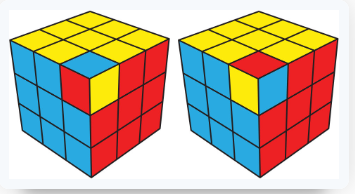
\includegraphics{Screenshot from 2024-03-24 08-41-47-1.png}
    %   \caption{Corner twist}
    % \end{figure}

  \end{block}

  \begin{block}{An algorithm for solving the Rubik's Cube}

    Nulla eget sem quam. Ut aliquam volutpat nisi vestibulum convallis. Nunc a
    lectus et eros facilisis hendrerit eu non urna. Interdum et malesuada fames
    ac ante \textit{ipsum primis} in faucibus. Etiam sit amet velit eget sem
    euismod tristique. Praesent enim erat, porta vel mattis sed, pharetra sed
    ipsum. Morbi commodo condimentum massa, \textit{tempus venenatis} massa
    hendrerit quis. Maecenas sed porta est. Praesent mollis interdum lectus,
    sit amet sollicitudin risus tincidunt non.

    Etiam sit amet tempus lorem, aliquet condimentum velit. Donec et nibh
    consequat, sagittis ex eget, dictum orci. Etiam quis semper ante. Ut eu
    mauris purus. Proin nec consectetur ligula. Mauris pretium molestie
    ullamcorper. Integer nisi neque, aliquet et odio non, sagittis porta justo.

    \begin{itemize}
      \item \textbf{Sed consequat} id ante vel efficitur. Praesent congue massa
        sed est scelerisque, elementum mollis augue iaculis.
        \begin{itemize}
          \item In sed est finibus, vulputate
            nunc gravida, pulvinar lorem. In maximus nunc dolor, sed auctor eros
            porttitor quis.
          \item Fusce ornare dignissim nisi. Nam sit amet risus vel lacus
            tempor tincidunt eu a arcu.
          \item Donec rhoncus vestibulum erat, quis aliquam leo
            gravida egestas.
        \end{itemize}
      \item \textbf{Sed luctus, elit sit amet} dictum maximus, diam dolor
        faucibus purus, sed lobortis justo erat id turpis.
      \item \textbf{Pellentesque facilisis dolor in leo} bibendum congue.
        Maecenas congue finibus justo, vitae eleifend urna facilisis at.
    \end{itemize}

  \end{block}

\end{column}

\separatorcolumn

\begin{column}{\colwidth}

  \begin{exampleblock}{A highlighted block containing some math}

    A different kind of highlighted block.

    $$
    \int_{-\infty}^{\infty} e^{-x^2}\,dx = \sqrt{\pi}
    $$

    Interdum et malesuada fames $\{1, 4, 9, \ldots\}$ ac ante ipsum primis in
    faucibus. Cras eleifend dolor eu nulla suscipit suscipit. Sed lobortis non
    felis id vulputate.

    \heading{A heading inside a block}

    Praesent consectetur mi $x^2 + y^2$ metus, nec vestibulum justo viverra
    nec. Proin eget nulla pretium, egestas magna aliquam, mollis neque. Vivamus
    dictum $\mathbf{u}^\intercal\mathbf{v}$ sagittis odio, vel porta erat
    congue sed. Maecenas ut dolor quis arcu auctor porttitor.

    \heading{Another heading inside a block}

    Sed augue erat, scelerisque a purus ultricies, placerat porttitor neque.
    Donec $P(y \mid x)$ fermentum consectetur $\nabla_x P(y \mid x)$ sapien
    sagittis egestas. Duis eget leo euismod nunc viverra imperdiet nec id
    justo.

  \end{exampleblock}

  \begin{block}{Nullam vel erat at velit convallis laoreet}

    Class aptent taciti sociosqu ad litora torquent per conubia nostra, per
    inceptos himenaeos. Phasellus libero enim, gravida sed erat sit amet,
    scelerisque congue diam. Fusce dapibus dui ut augue pulvinar iaculis.

    \begin{table}
      \centering
      \begin{tabular}{l r r c}
        \toprule
        \textbf{First column} & \textbf{Second column} & \textbf{Third column} & \textbf{Fourth} \\
        \midrule
        Foo & 13.37 & 384,394 & $\alpha$ \\
        Bar & 2.17 & 1,392 & $\beta$ \\
        Baz & 3.14 & 83,742 & $\delta$ \\
        Qux & 7.59 & 974 & $\gamma$ \\
        \bottomrule
      \end{tabular}
      \caption{A table caption.}
    \end{table}

    Donec quis posuere ligula. Nunc feugiat elit a mi malesuada consequat. Sed
    imperdiet augue ac nibh aliquet tristique. Aenean eu tortor vulputate,
    eleifend lorem in, dictum urna. Proin auctor ante in augue tincidunt
    tempor. Proin pellentesque vulputate odio, ac gravida nulla posuere
    efficitur. Aenean at velit vel dolor blandit molestie. Mauris laoreet
    commodo quam, non luctus nibh ullamcorper in. Class aptent taciti sociosqu
    ad litora torquent per conubia nostra, per inceptos himenaeos.

    Nulla varius finibus volutpat. Mauris molestie lorem tincidunt, iaculis
    libero at, gravida ante. Phasellus at felis eu neque suscipit suscipit.
    Integer ullamcorper, dui nec pretium ornare, urna dolor consequat libero,
    in feugiat elit lorem euismod lacus. Pellentesque sit amet dolor mollis,
    auctor urna non, tempus sem.

  \end{block}

  \begin{block}{References}

    \nocite{*}
    \footnotesize{\bibliographystyle{plain}\bibliography{poster}}

  \end{block}

\end{column}

\separatorcolumn
\end{columns}
\end{frame}

\end{document}
